After a user application has obtained an OutComponent component from an OutFactory, it loads it into the OutLoader. This component is responsible for selecting the appropriate OutManager to process the out-going command or report.

For this purpose, the OutLoader maintains a list of OutManagers (the List of OutManagers or LOM). The LOM holds all the OutManagers which have been instantiated in an application. 

The OutLoader component offers one operation – the \texttt{Load} operation – to load an OutComponent into an OutManager. When this operation is called, the OutLoader decides to which OutManager in the LOM to load an OutComponent. The policy for selecting the OutManager in the LOM is an adaptation point. After the OutComponent is loaded into the selected OutManager, the procedure may activate the selected OutManager (i.e. it may release the thread which is controlling the execution of the selected OutManager). This is useful where there is a need to process the out-going command or report as soon as it is loaded into the OutLoader (normally, the command or report would only be processed when the OutManager is executed). 
 
The \texttt{Load} operation is modelled by the procedure shown in figure \ref{fig:OutLoaderLoad}. A call to operation \texttt{Load} causes this procedure to be started and executed. The procedure executes in one single cycle and therefore terminates as part of the call to operation \texttt{Load}. 

No facilities are defined for dynamically changing the set of OutManagers in the LOM. Changes in the list of OutManagers can only be done by reconfiguring and then resetting the OutLoader component.

\begin{figure}[h]
 \centering
 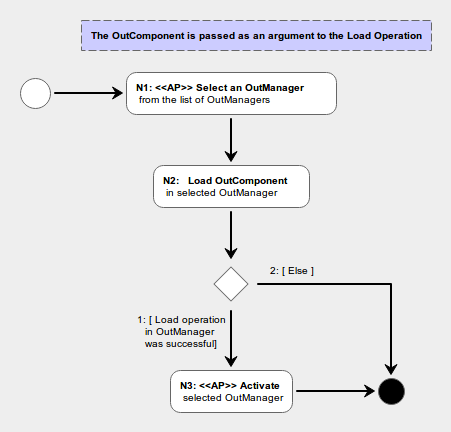
\includegraphics[scale=0.40,keepaspectratio=true]{OutLoaderLoad.png}
 \caption{The OutLoader Load Procedure}
 \label{fig:OutLoaderLoad}
\end{figure}
